\section{Introduction}
Let $(X,g)$ be a space-time and $p\in X$.  One structure that can be associated to a space-time is the space $\mathcal{N}$ of all light rays on the manifold.    To a point $p$ in the manifold one associates the sphere in $\mathcal{N}$ of light rays passing through $p$, which we call its \emph{sky} and denote by $\mathcal{O}_p$.  The space of all skies is called the \emph{sky space} of $X$ and is denoted $SKY(X)$.  The two statements of refocusing address  properties of the mapping $p\rightarrow \mathcal{O}_p$.  If a space-time is not strongly refocusing then the map is injective.  Furthermore if a strongly causal $X$ is not refocusing Low \cite{LowNull} showed that the map is a diffeomorphism.

The definition of refocusing was first formulated by Low when he was studying the space of light rays on a space-time.  In fact, he proposed three definitions of refocusing in \cite{LowCS}, \cite{LowSS} and \cite{LowNull}.  The proof of the statement that these definitions are equivalent can be found in the work of Kinlaw \cite{Kinlaw}.  This established the definition of refocusing that we will use in this paper.

After establishing the definitions it is natural to consider whether examples exist of space-times that are strongly refocusing but not refocusing.  In this paper we prove the following result:

\begin{prop} \label{mainProp}
A $1+1$-dimensional oriented, time oriented, refocusing space-time is also strongly refocusing.
\end{prop}

Other questions in the same line were previously explored by Kinlaw \cite{Kinlaw}.  He constructed the first example of a globally hyperbolic space-time which is refocusing but not strongly refocusing at every point in a Cauchy surface.  Using the Poincare conjecture proved by Perlman, he was also able to prove that any globally hyperbolic refocusing space-time of dimension $\leq 4$ admits a strongly refocusing metric.

These results provide the basis for our investigation.  They also aim to answer if and when there are examples of space-times that are refocusing but are not strongly refocusing.

\section{Definitions} 
In this section we will provide the definitions that we use throughout the paper.  We begin with the definitions of strong refocusing and refocusing.
\begin{defin} \label{srefoc}
A space-time $(X, g)$ is \emph{strongly refocusing} at $p\in X$ if there exists $q\neq p \in X$ such that all the light rays passing through $q$ also pass through $p$.  We say $X$ is \emph{strongly refocusing} if there exists $p\in X$ such that $X$ is strongly refocusing at $p$.
\end{defin}

\begin{rem}
In Low's work refocusing was considered only for strongly causal space-times.  In this work we do not use this assumption.
\end{rem}

In order to define refocusing we weaken the conditions of strong refocusing.  Low initially proposed three definitions for refocusing, and for strongly causal space-times they were proven to be equivalent by Kinlaw \cite{Kinlaw}.  We will use the following definition:
\begin{defin} \label{refoc}
A space-time $(X, g)$ is \emph{refocusing} at $p\in X$ if there exists an open neighborhood $V$ of $p$ such that for all open $U\subset V$ with $x\in U$ there exists $y\notin V$ such that all null geodesics passing through $y$ also pass through $U$.
\end{defin}

From these definitions it is clear that any strongly refocusing space-time is also refocusing.


\subsection{Right and Left Null Geodesics}
For a $2-$dimensional oriented, time-oriented space-time $X$, each null geodesic in $X$ can be classified into one of two types.  Let $\gamma$ be a null geodesic, and let $Y$ be any timelike future pointing vector field.  The pair $\gamma '(t)$ and $Y(\gamma(t))$ are linearly independent, and thus form a basis for $T_{\gamma(t)}X$ for any $p\in X$. Let $X_1$ and $X_2$ be vector fields that orient $X$, and for two bases of $T_p X$, $\{v_1, v_2\}$ and $\{w_1, w_2\}$, denote by $_{\{w_1, w_2\}}M_{\{v_1, v_2\}}$ the change of basis matrix from $\{v_1, v_2\}$ to $\{w_1, w_2\}$.  At $\gamma(t)$ we have two bases of $T_{\gamma(t)} X$:$\{\gamma '(t), Y(\gamma(t))\}$ and $\{X_1(\gamma(t)), X_2(\gamma(t))\}$.  Define a function to measure whether these two bases define the same orientation of $T_{\gamma(t)} X$ as follows:

$$f_\gamma(t) = \mbox{det}\left( _{\{\gamma '(t), Y(\gamma(t))\}}M_{\{X_1(\gamma(t)), X_2(\gamma(t))\}} \right)$$

Note that $f$ is continuous and identifies whether the orientation defined by the basis $\gamma '(t)$ and $Y(\gamma(t))$  agrees or disagrees with the orientation given by $X_1$ and $X_2$.  Since this function is never zero (as the change of basis matrix is always non-degenerate) it must be always positive or always negative.  

\begin{defin}
Let $\gamma$ be a null geodesic of $X$.  We say that $\gamma$ is \emph{left-facing} if $f_\gamma(t) < 0$ for all $t$ and \emph{right-facing} if $f_\gamma(t) > 0$ for all $t$. 
\end{defin}

\begin{rem}
\begin{enumerate}
\item Every null geodesic is either left facing or right facing.
\item Each point $p\in X$ has exactly two null geodesics passing through it, one of which is left facing and one of which is right facing.  We denote by $\rho_x$ the right facing null geodesic starting at $x$ and by $\lambda_x$ the left facing null geodesic starting at $x$.
\item It is impossible for two right-facing or two left-facing geodesics to intersect.
\end{enumerate}
\end{rem}



\section{Proof of \ref{mainProp}}
In this section we will prove Proposition \ref{mainProp}.  Throughout the section let $(X, g)$ be an oriented, time-oriented $1+1$ dimensional space-time.  Recall that for any $p,q\in X$, $I^\pm(p)$ denotes the chronological future/past of $p$ and $I(p,q) = I^+p \cap I^-q$.

%As remarked above it is clear that if $X$ is strongly refocusing then it is also refocusing.

Suppose that we have refocusing at $x\in X$.  Again, let $Y$ be a future facing timelike vector field on $X$.  Since $X$ is refocusing at $x$ we have a neighborhood $W$ of $x$ such that for any open $U\subset W$ with $x\in U$ there exists $y\notin W$ where all the null geodesics passing through $y$ also pass through $V$.  

We begin by constructing a neighborhood of $x$ where we will force strong refocusing to occur.  Let $(V, \psi)$ be a globally hyperbolic, normal coordinate neighborhood of $x$ such that $V\subset W$ and for fixed $c$ the curves $\gamma_c(t) = \psi^{-1}(c, t)$ are integral curves of $Y$. We may also assume that the local frame given by the coordinate vector fields $\{\partial \phi_1$,$\partial\phi_2\}$ agrees with the orientation on $X$.  

Now choose $z_0, z_1 \in V$ such that $x\in I(z_0, z_1)$ and $\overline{I(z_0, z_1)} \subset V$.  Note that $I(z_0, z_1)$ is an open neighborhood of $x$ with boundary formed by the left facing null geodesics $\lambda_{z_0}$ and $\lambda_{z_1}$ and right facing geodesics $\rho_{z_0}$ and $\rho_{z_1}$.  This neighborhood is depicted in Figure  \ref{figure1.fig}.

\begin{figure}[htbp]
	\centering
	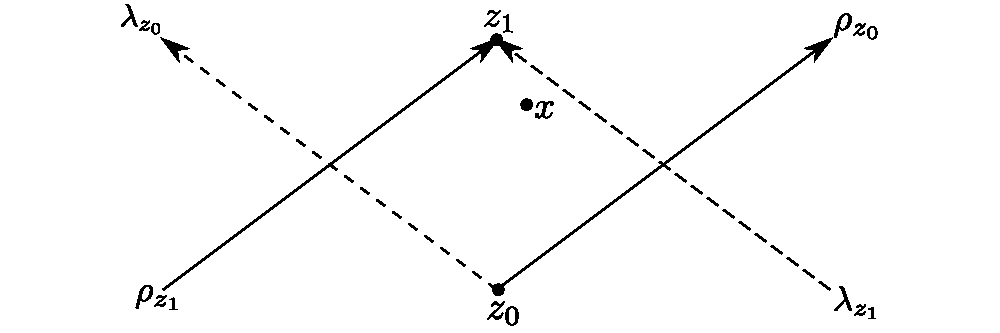
\includegraphics[width=12cm]{simpleRefocussingNbhd}
	\caption{A diagram of $I(z_0, z_1)$}
	\label{figure1.fig}
\end{figure}

Now we show that there must be strong refocusing in $V$.

Since that $X$ is refocusing at $x$ and $I(z_0, z_1)\subset W$, we may choose $y\notin W$ such that $p = \lambda_y (t_0) \in \mbox{Im}(\lambda_y) \cap I(z_0, z_1)$ and $q = \rho_y (t_1) \in \mbox{Im}(\rho_y) \cap I(z_0, z_1)$.  To show that there is strong refocusing on $X$ we will show that either $\lambda_y$ intersects $\rho_y$, or strong refocusing occurs elsewhere in $V$.  
%(Here $I^\pm(p)$ is the chronological future/past of $p$.)  Then $\psi(V)$ contains a diagram similar to the one illustrated in Figure \ref{figure1.fig}.  Finally choose $a,b,c$ and $d$ so that $\rho_p([-a, 0])$, $\lambda_p([-b, 0])$, $\rho_q([0, c])$ and $\lambda_q([0, d])$ form the boundary of $I^-(p)\cap I^+(q)$.

 

\begin{figure}[hbtp]
	\centering
	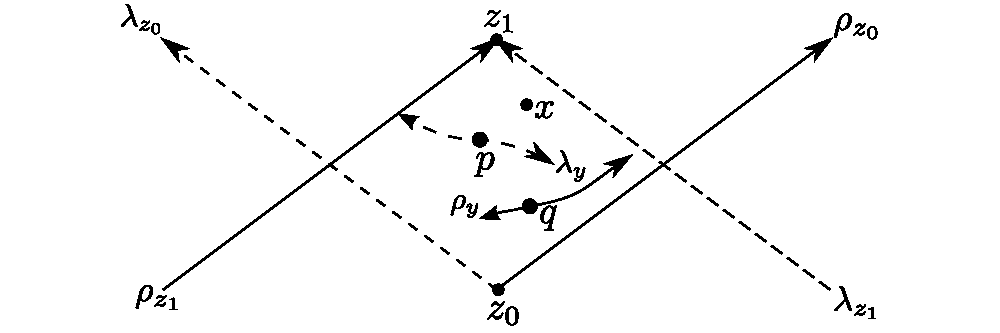
\includegraphics[width=12cm]{refocussingNbhd}
	\caption{A diagram of $I(z_0, z_1)$}
	\label{figure2.fig}
\end{figure}

As $I(z_0, z_1)$ is in the interior of a normal neighborhood of $x$ we must have that the future (resp. past) progression of $\rho_y$ from $q$ intersects $\partial I(z_0, z_1)$ at a point $b$ (resp $a$).  Since $\rho_y$ is right facing it cannot intersect $\rho_{z_0}$ or $\rho_{z_1}$.  Suppose $a$ and $b$ are both contained in $\mbox{Im}(\lambda_{z_0})$.  Then both light rays passing through $a$ would also pass through $b$, so we would have strong refocusing of $X$ at $a$ and would be done.  In order to avoid strong refocusing $\rho_y$ must intersect both $\mbox{Im}(\lambda_{z_0})$ and $\mbox{Im}(\lambda_{z_1})$.

Similarly to avoid strong refocusing when considering the past and future progression of $\lambda_y$ from $p$ we must have that $\lambda_y$ intersects both $\mbox{Im}(\rho_{z_0})$ and $\mbox{Im}(\rho_{z_1})$.  However to connect these pairs of points $\rho_q$ must intersect $\lambda_p$ in $I(z_0, z_1)$ and hence we have that $X$ is strongly refocusing at $y$.

\begin{rem}
All known examples of refocusing higher dimensional space-times are also strongly refocusing.  Whether this is always the case remains an open question.
\end{rem}


%\section{Introduction}
%In this section our goal is to reach our results on refocussing in two dimensional Lorentz manifolds.  With that in mind we will begin by providing a background in Lorentz geometry.  Then we give the definition and some examples of refocussing and strongly refocussing Lorentz manifolds.  We conclude by proving that the notions of refocussing and strong refocussing are equivalent for oriented, two dimensional Lorentz manifolds.
%\subsection{Lorentz Manifolds}
%Let $M$ be a smooth manifold of dimension $n$.  A \emph{semi-Riemannian metric} on $M$ is a non-degenerate $(2,0)$-tensor field on $M$, or equivalently a \emph{metric} is a choice of non-degenerate symmetric bilinear form $g:T_p M \times T_p M \rightarrow \mathbb{R}$ for all $p \in M$ that varies smoothly with $p$.  
%
%Since the matrix of a semi-Riemannian metric $g$ at a point $p$ is symmetric it can be diagonalized with respect to some basis in $T_pM$.  Furthermore, since $g$ is non-degenerate we know that 0 is not an eigenvalue.  Thus the matrix of the metric at a point can be represented as the $\mbox{diag}(1,\dots, 1, -1, \dots, -1)$, where $-1$ appears $k$ times and $1$ appears $n-k$ times for some $0\leq k \leq n$.  The \emph{signature} of a metric is given by the vector $(1,\dots, 1, -1, \dots, -1)$.  The \emph{index} of a metric is $k$.  It is not immediately clear that the index is well defined, but Sylvester's Law of Inertia (see \ref{smlgb}) guarantees that the index is independent of the choice of basis.  It can be shown that the index of a metric is a smooth function on a $M$ that takes values in $\mathbb{Z}$ and therefore is constant on the connected components of $M$.
%
%\begin{rem}
%A \emph{Riemannian metric} on a manifold is a semi-Riemannian metric of index 0.  A \emph{Lorentz metric} is a semi-Riemannian metric of index $1$.  Finally, a \emph{Lorentz manifold} $(M, g)$ is a smooth manifold $M$ equipped with a Lorentz metric $g$.
%\end{rem}
%\subsection{The null-cone}
%The metric of a Lorentz manifold can be used to decompose the tangent space at a point into 3 disjoint sets.  Given a Lorentz manifold $(M, g)$ and a vector $v\in T_p M$ we can define the \emph{causal character} of $v$ as follows:
%\begin{defin}
%Let $(M, g)$ be a Lorentz manifold, $p\in M$ and $v\neq \mathbf{0} \in T_p M$.  If $g_p(v,v) < 0$ we say that the causal character of $v$ is \emph{timelike} (more frequently we simply say $v$ is timelike).  Similarly if $g_p(v,v) < 0$  we call $v$ \emph{spacelike}.  Finally if $g_p(v,v) = 0$ we call $v$ a \emph{lightlike} vector or a \emph{null} vector.
%\end{defin}
%
%These definitions can also be extended to smooth curves as follows.  Given a smooth curve $\gamma:\mathbb{R}\rightarrow M$, we call $\gamma$ \emph{timelike} (resp. \emph{spacelike}, \emph{lightlike} if $g_{\gamma(t)}(\gamma '(t), \gamma '(t))$ is negative (resp. positive, zero) for all $t$.  We can also extend them to submanifolds.  A smooth submanifold $N\subset M$ is called \emph{spacelike} if $g|N$ is Riemannian.
%
%We can apply this definition to the geodesics of $M$.  Given $v\in T_p M$ we can look at the unique geodesic $\gamma_p$ of $M$ tangent to $v$ at $p$.  Note that since $\gamma_p$ is a geodesic it must always have the same causal character. 
%
%\begin{defin}
%The \emph{null-cone} at $p$, denoted $N_p$ is the set of all null vectors at $p$.  It is important to note that $N_p$ is a subset of $T_p M$, but not a subspace, as $0 \notin N_p$.  It consists of two disconnected hemicones emanating from the origin.  
%\end{defin}
%
%The exponentiated null-cone is sometimes also called the null-cone.  We will follow that convention where it is clear from context which version is intended.  
%
%\subsection{Conformal Equivalence}
%Many interesting properties of a Lorentz manifold are preserved when the metric is scaled by a positive constant.  Given a Lorentz manifold $(M,g)$ a conformal factor is a function $\Omega : M \rightarrow \mathbb{R}^+$.
%\begin{defin}
%Let $M$ be a smooth manifold and $g$ and $g'$ be Lorentz metrics on $M$.  The metrics $g$ and $g'$ are \emph{conformally equivalent} if there exists a conformal factor $\Omega$ such that $g = \Omega g'$.
%\end{defin}
%
%Notice that the conformal character of a vector is the same for all conformally equivalent metrics.  Thus, the conformal character of curves remains the same if the metric is changed by a conformal factor.  Furthermore, the null-cone and the exponentiated null-cone are both invariant under conformal change of the metric.    
%
%\subsection{Time orientability}
%
%\subsection{The causal structure of spacetimes?}
%
%\subsection{The space $\mathcal{N}$ of Null geodesics}
%The invariance of the causal structure of a Lorentz manifold under conformal change of the metric suggests that there may be a more appropriate structure related to a Lorentz manifold to consider when investigating issues of causality.  The space $\mathcal{N}$ of null geodesics was introduced by Robert Low in his 
%
%
%\subsection{Refocussing and Strong Refocussing}
%\subsection{Results in 2-dimensional spacetimes}
%If $(X,g)$ is a globally hyperbolic 2-dimensional oriented, time-oriented Lorentzian manifold then we can classify the null geodesics according to the orientation that their velocity vector and the time orienting vector induce at a point on the manifold. In particular if $Y$ is a non-zero future oriented timelike vector field and $\gamma$ is a null geodesic then the pair $\gamma '(t)$ and $Y(\gamma(t))$ are linearly independent, and thus form a basis for $T_pX$. If $X_1$ and $X_2$ are vector fields that orient X and then the function
%
%$$f_\gamma(t) = \mbox{det}\left(
%\begin{array}{cc}
%X_1(\gamma(t)) & X_2(\gamma(t))\\
%\gamma '(t) & Y(\gamma(t))
%\end{array}
%\right)
%$$
%is continuous and tells whether $\gamma '(t)$ and $Y(\gamma(t))$ give the correct orientation or the reversed orientation. Note that since this function is continuous on the domain of the geodesic and is never zero it must be either always positive or always negative. Call $\gamma$ left-facing if $f_\gamma(t) < 0$ and right-facing if $f_\gamma(t) > 0$. Note that this classification of geodesics also tells us that it is impossible for two right-facing or two left-facing geodesics to intersect, as at each point there are exactly two null-geodesics passing through one of which must be left-facing and one right-facing. 
%
%Now suppose that we have weak refocusing at $x\in X$. Let $V$ be a coordinate neighborhood of $x$ with integral curves of $Y$ as the second coordinate. Let $x\in U \subset V$ be a convex normal neighborhood of $x$. Finally let $p \in U$ with $x \in I^-(p)$ and $q \in U$ with $x \in I^+(q)$. Then our coordinate neighborhood contains a picture that looks like this:
%
%
%
%In all diagrams left-facing null geodesics are in red and right-facing null-geodesics are in black. In this figure we have an $x$ coordinate and the y-coordinate corresponds to time, since we chose our coordinates in this way.  Now, since our manifold is refocusing we know that there is a point, $z$, whose null cone lies inside this diamond. Since our manifold is globally hyperbolic we may assume $X = M \times \mathbb{R}$ and $x = (m, t_0)$. Now look at the points where the null cone of $z$ intersects the Cauchy surface $M \times \{ t_0 \}$. Call the point of intersection with smaller first coordinate $a$ and the point with larger first coordinate $b$. Call the null geodesic from $z$ to $a$ $\gamma_a$ and the null geodesic from $z$ to $b$ $\gamma_b$. Now there are two possibilites, either $\gamma_a$ is left-facing and $\gamma_b$ is right-facing or vice-versa.
%
%Lets consider the case when $\gamma_a$ is left-facing and $\gamma_b$ is right-facing. We can look at the progression backwards in time of 
%$\gamma_b$ from $b$. Note that in coordinates its $t$ coordinate must be decreasing and also it cannot cross the right-facing null geodesic leaving $q$. Thus it must intersect the left-facing geodesic leaving $q$, so $\gamma_b$, the left-facing geodesic leaving $q$ and the Cauchy
%surface $M \times \{t_0\}$ form a triangle. $a$ lies on this triangle and the progression backwards in time
%of $\gamma_a$ must enter this triangle. So we have the following situation:
%
%
%Now consider the possibilities for the backward progression of $\gamma_a$. To leave the triangle it
%must intersect either (i) the left facing null geodesic leaving q, (ii) the Cauchy surface $M \times \{t_0\}$, or
%(iii) $\gamma_b$.
%b. Cases (i) and (ii) are impossible, so (iii) must occur giving us strong refocusing at the
%point of intersection of $\gamma_a$ and $\gamma_b$. Thus if we have the case where $\gamma_a$ is left-facing and $\gamma_b$ is
%right-facing we must have strong refocusing.
%
%
%So lets consider the case where $\gamma_a$ is left-facing and $\gamma_b$ is right-facing. Well, this case turns into exactly the same situation when you consider the forward time progression of the geodesics instead of the backward time progression.  Thus in a 2-dimensional globally hyperbolic oriented, time-oriented Lorentzian manifold weak refocusing implies strong refocusing.